

\begin{frame}
	\titlepage
\end{frame}

\begin{frame}{Технология маячков}
	\begin{figure}
		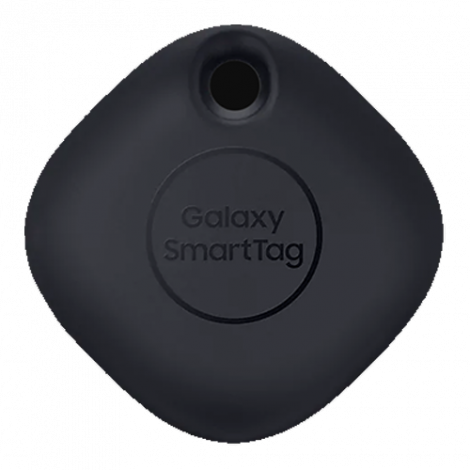
\includegraphics[width=0.15\linewidth]{images/beacon.png}
	\end{figure}
	\textbf{Bluetooth-маячок} - устройство, транслирующее с интервалом пакеты 
	стандарта Bluetooth LE.
	
	Особенности:
	\begin{enumerate}
		\item Малый размер
		\item Невысокая стоймость (3-10\$)
		\item Низкое энергопотребление: может работать годами без замены батареи
	\end{enumerate}
\end{frame}

\begin{frame}{Применения маячков}
	\begin{enumerate}
		\item Уведомление пользователей
		\item Пересылка информации: измеренные температура и давление
		\item Навигация внутри помещения
	\end{enumerate}
\end{frame}

\begin{frame}{Как работает навигация?}
	\begin{itemize}
		\item Каждый интервал времени маячок отсылает Measured Power (уровень сигнала в 1 м от передатчика, \textit{dBm}).
		\item Приемник измеряет уровень приходящего сигнала в \textit{dBm}. 
		\item Двух этих величин достаточно, чтобы определить расстояние от приемника до передатчика.
		\item Имея несколько передатчиков и зная их позиции, можно определить местоположение принимающего устойства.
	\end{itemize}
\end{frame}

\begin{frame}{Концепция}
	\begin{itemize}
		\item Отслеживая местоположение работников на предприятии,
		можно эффективнее распределять задачи между ними.
		\item Может быть полезно в поиске "узких мест" в производственном процессе.
	\end{itemize}
	
\end{frame}

\begin{frame}{Задачи}
	
	\begin{enumerate}
		\item Исследование предметной области.
	
		\item Определение требований к системе.
	
		\item Анализ существующих технологий и программных комплексов и их сравнение.
	
		\item Выбор программных комплексов.
	
		\item Разработка архитектуры программного комплекса и систем.
	
	\end{enumerate}
\end{frame}

\begin{frame}{Акторы}
	\begin{enumerate}
		\item Рабочие
		\item Управляющие
		\item Администратор системы
	\end{enumerate}
	Требования:
	\begin{enumerate}
		\item Масштабируемость
		\item Возможность интеграции с существующими системами
	\end{enumerate}
\end{frame}

\begin{frame}{Система}
	\begin{figure}
		\includegraphics[width=0.65\linewidth]{images/beacon-sys.png}
		\caption{Система}
	\end{figure}
\end{frame}

\begin{frame}{Подбор программых комплексов}
	\begin{enumerate}
		[]\item 
		\begin{figure}
			
\includegraphics[width=0.4\linewidth]{images/jira_software.png}
		\end{figure}
		Пользовательский интерфейс и управление задачами 
		(в какой-то степени) - \textbf{Jira}
		
		\textit{Причины:} Jira уже используется на предприятиях.
		Позиционирование сотрудников будет проще интегрировать в уже
		развернутые системы. 
		
	\end{enumerate}
\end{frame}

\begin{frame}{Подбор программых комплексов}
	\begin{enumerate}
		[]\item 
		\begin{figure}
			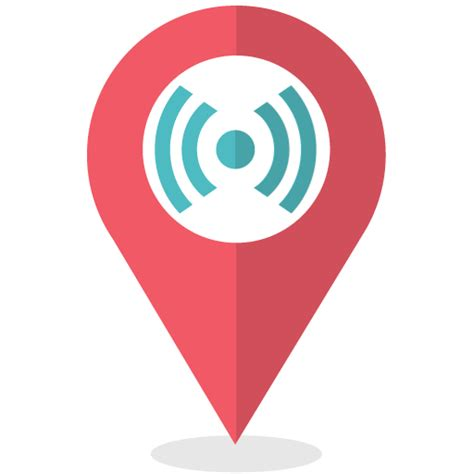
\includegraphics[width=0.15\linewidth]{images/find3.png}
		\end{figure}
		Система позиционирования - \textbf{FIND3} Framework 
		
		\textit{Причины:} бесплатен, открытый код
	\end{enumerate}
\end{frame}

\begin{frame}{Результаты}
	\begin{enumerate}
		\item Изучена предметная область работы.
		\item Определены требования к системе.
		\item Проведен анализ и выбор программных комплексов 
		\item Разработана архитектура системы.
	\end{enumerate}
\end{frame}

	